\documentclass[a4paper]{article}
\usepackage[utf8]{inputenc}
\usepackage[catalan]{babel}
\usepackage{listings}
\usepackage[svgnames]{xcolor}
\usepackage{graphicx}


\lstset{language=R,
    basicstyle=\small\ttfamily,
    stringstyle=\color{DarkGreen},
    otherkeywords={0,1,2,3,4,5,6,7,8,9},
    morekeywords={TRUE,FALSE},
    deletekeywords={data,frame,length,as,character},
    keywordstyle=\color{blue},
    commentstyle=\color{DarkGreen},
}

\author{
Gerard Barrachina
\and
Josep de Cid
\and
Albert Ribes
\and
Kerstin Winter
}

\title{Problema 3: Interacció entre partícules [R, G]}

\begin{document}
\maketitle

S'ha dissenyat un experiment per provar una teoria sobre la naturalesa de la interacció entre certs tipus
de partícules elementals en col·lisió amb protons. Es creu que la secció transversal està linealment
relacionada amb la inversa de l'energia. A tal efecte, s'han determinat submostres per diferents nivells
de la inèrcia de la partícula. En cada submostra es van prendre un gran nombre d'observacions i això ha
permès estimar la desviació estàndar (sd) de la secció transversal (st) mesurada, com indica la Taula 1.

\begin{center}
\begin{tabular}{c c c}

  \textit{energia} & \textit{st} & \textit{sd} \\
  2.899 & 367 & 17 \\
  3.484 & 311 & 9 \\
  3.984 & 295 & 9 \\
  4.444 & 268 & 7 \\
  4.831 & 253 & 7 \\
  5.376 & 239 & 6 \\
  6.211 & 220 & 6 \\
  7.576 & 213 & 6 \\
  11.905 & 193 & 5 \\
  16.667 & 192 & 5 \\
\end{tabular}
\end{center}

Plantegeu el problema de predir la secció transversal amb la inversa de l'energia com una regressió
lineal ponderada (vegeu el problema 7 del TEMA 1). Resoleu-lo numèricament usant la rutina \texttt{lm()} (ó
\texttt{glm()} si especifiqueu \texttt{family=gaussian)}. Feu un gràfic del resultat amb i sense la ponderació; compareu
els resultat i expliqueu la raó de les diferències.

\hspace{5cm}

\textbf{
Hay que dar menos peso a los datos que tengan una varianza más grande. Por eso
hemos establecido que el peso será el inverso de la varianza. Como los datos
solo nos dan la desviación estándar, hay que elevarlo al cuadrado.
}

\textbf{Viendo el gráfico \ref{f1} da la impresión de que el modelo que asume
homocedasticidad se adapta mejor a los datos. Pero esto es normal, ya que se
está adaptando por igual a los valores menos y más plausibles.}

\textbf{La recta roja está más cerca de los puntos con valores de st alrededor
de 250, que son los que menos varianza tienen y por lo tanto más seguros}


\begin{center}
\begin{figure}[h]
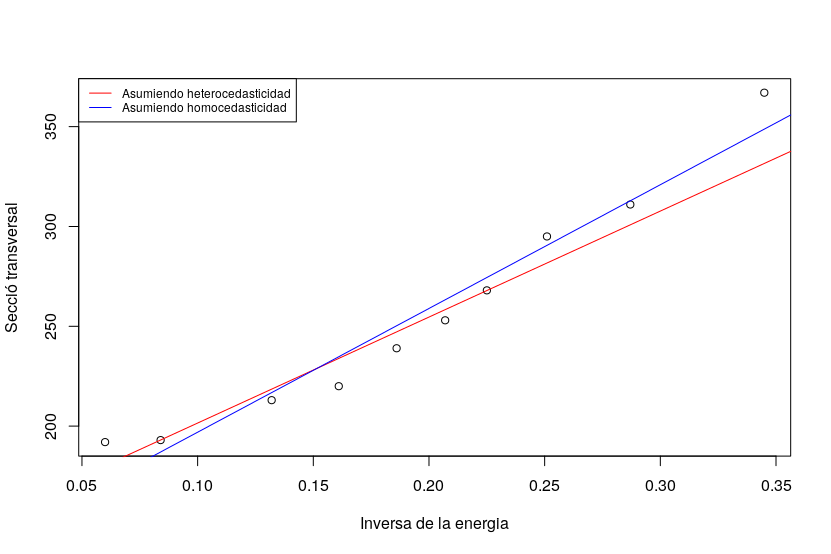
\includegraphics[width=8cm]{plot}
\caption{Predicción del modelo}
\label{f1}
\end{figure}
\end{center}


\begin{lstlisting}
energy = c(
          2.899,
          3.484 ,
          3.984 ,
          4.444 ,
          4.831 ,
          5.376 ,
          6.211 ,
          7.576 ,
          11.905 ,
          16.667
)

st = c(
       367 ,
       311 ,
       295 ,
       268 ,
       253 ,
       239 ,
       220 ,
       213 ,
       193 ,
       192
)

sd = c(
       17,
       9,
       9,
       7,
       7,
       6,
       6,
       6,
       5,
       5
)

energy.inv = 1/energy
var = sd^2
w = 1 / var

df = data.frame(energy.inv, st)

l.heter = lm(formula = st ~ energy.inv, weights = w, data = df)
l.homo = lm(formula = st ~ energy.inv, data = df)



plot(energy, inv.st,ylab = "Seccio transversal", xlab = "Inversa de la energia")
legend('topleft', c("Asumiendo heterocedasticidad","Asumiendo homocedasticidad")
 , lty=1, col=c('red', 'blue'), bty='L', cex=.75)
abline(l.heter$coefficients[1], l.heter$coefficients[2], col = "red")
abline(l.homo$coefficients[1], l.homo$coefficients[2], col = "blue")



\end{lstlisting}


\end{document}
